\PassOptionsToPackage{unicode=true}{hyperref} % options for packages loaded elsewhere
\PassOptionsToPackage{hyphens}{url}
%
\documentclass[]{article}
\usepackage{lmodern}
\usepackage{amssymb,amsmath}
\usepackage{ifxetex,ifluatex}
\usepackage{fixltx2e} % provides \textsubscript
\ifnum 0\ifxetex 1\fi\ifluatex 1\fi=0 % if pdftex
  \usepackage[T1]{fontenc}
  \usepackage[utf8]{inputenc}
  \usepackage{textcomp} % provides euro and other symbols
\else % if luatex or xelatex
  \usepackage{unicode-math}
  \defaultfontfeatures{Ligatures=TeX,Scale=MatchLowercase}
\fi
% use upquote if available, for straight quotes in verbatim environments
\IfFileExists{upquote.sty}{\usepackage{upquote}}{}
% use microtype if available
\IfFileExists{microtype.sty}{%
\usepackage[]{microtype}
\UseMicrotypeSet[protrusion]{basicmath} % disable protrusion for tt fonts
}{}
\IfFileExists{parskip.sty}{%
\usepackage{parskip}
}{% else
\setlength{\parindent}{0pt}
\setlength{\parskip}{6pt plus 2pt minus 1pt}
}
\usepackage{hyperref}
\hypersetup{
            pdftitle={Data description},
            pdfauthor={Daiga Paršova},
            pdfborder={0 0 0},
            breaklinks=true}
\urlstyle{same}  % don't use monospace font for urls
\usepackage[margin=1in]{geometry}
\usepackage{graphicx,grffile}
\makeatletter
\def\maxwidth{\ifdim\Gin@nat@width>\linewidth\linewidth\else\Gin@nat@width\fi}
\def\maxheight{\ifdim\Gin@nat@height>\textheight\textheight\else\Gin@nat@height\fi}
\makeatother
% Scale images if necessary, so that they will not overflow the page
% margins by default, and it is still possible to overwrite the defaults
% using explicit options in \includegraphics[width, height, ...]{}
\setkeys{Gin}{width=\maxwidth,height=\maxheight,keepaspectratio}
\setlength{\emergencystretch}{3em}  % prevent overfull lines
\providecommand{\tightlist}{%
  \setlength{\itemsep}{0pt}\setlength{\parskip}{0pt}}
\setcounter{secnumdepth}{0}
% Redefines (sub)paragraphs to behave more like sections
\ifx\paragraph\undefined\else
\let\oldparagraph\paragraph
\renewcommand{\paragraph}[1]{\oldparagraph{#1}\mbox{}}
\fi
\ifx\subparagraph\undefined\else
\let\oldsubparagraph\subparagraph
\renewcommand{\subparagraph}[1]{\oldsubparagraph{#1}\mbox{}}
\fi

% set default figure placement to htbp
\makeatletter
\def\fps@figure{htbp}
\makeatother

\usepackage{etoolbox}
\makeatletter
\providecommand{\subtitle}[1]{% add subtitle to \maketitle
  \apptocmd{\@title}{\par {\large #1 \par}}{}{}
}
\makeatother
% https://github.com/rstudio/rmarkdown/issues/337
\let\rmarkdownfootnote\footnote%
\def\footnote{\protect\rmarkdownfootnote}

% https://github.com/rstudio/rmarkdown/pull/252
\usepackage{titling}
\setlength{\droptitle}{-2em}

\pretitle{\vspace{\droptitle}\centering\huge}
\posttitle{\par}

\preauthor{\centering\large\emph}
\postauthor{\par}

\predate{\centering\large\emph}
\postdate{\par}

\title{Data description}
\author{Daiga Paršova}
\date{11/28/2019}

\begin{document}
\maketitle

\hypertarget{phd-research-topic-and-objective}{%
\subsection{PhD research topic and
objective}\label{phd-research-topic-and-objective}}

The topic of the PhD research is ``Assessing the Spatiotemporal
Variability in Environmental Exposure''. The objective of the research
in 4 year period is to reach a better understanding of the associations
between urban mobility and environmental exposure via developing
methodology of assessing dynamic exposure to urban greenspaces and air
pollution.

\hypertarget{methods-and-software-availability}{%
\subsection{Methods and software
availability}\label{methods-and-software-availability}}

To develop the methodology of assessing dynamic exposure to urban
greenspaces, air pollution, and noise, geocomputational (share of land
use per area unit; functional density; aggregation of exposure, based on
time; temporal differences, etc.) and statistical methods will be
exploited.

\hypertarget{vizualization}{%
\subsection{Vizualization}\label{vizualization}}

The data vizualiations will be produced via open-source software.
However, it must be done in a way that particular individuals cannot be
recognized from the visualiation. On the other hand, if presenting the
whole dataset, it is a challenge to do it in understandable way. Below,
an example on Tartu bicycle sharing system is presented. These are bike
rides taking place in July, 2019. This data is available publicly. Each
color indicates a separate ride. However, it is not possible to
distinguish a separate route.

\begin{figure}
\centering
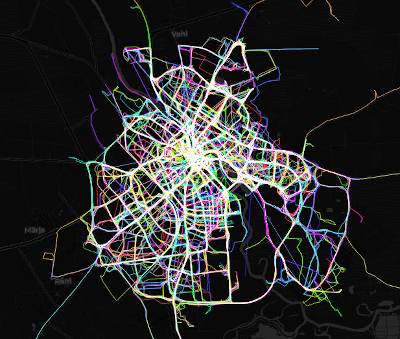
\includegraphics{Tartu_bikes.png}
\caption{GPS data vizualization example: Tartu bicycle sharing system}
\end{figure}

\hypertarget{reproducibility}{%
\subsection{Reproducibility}\label{reproducibility}}

\hypertarget{analysis}{%
\subsubsection{Analysis}\label{analysis}}

Geocomputational analysis will be conducted in PostgreSQL and QGIS.
Statistical analysis will be performed in RStudio. All of the software
used for the analysis is open-source. The code used for the analysis
will be available in a public repository and thus can be accessed and
modified if necessary.

\hypertarget{data}{%
\subsubsection{Data}\label{data}}

Long-term pseudonymized GPS dataset will be analyzed in relation to land
use and other environment characteristics. Fine scale (grid cell 25 m x
25 m) modeled air pollution and noise level data will be provided by the
Institute of Family Medicine and Public Health. Land cover data will be
retrieved from the Estonian Topographic Database and OpenStreetMap.

\hypertarget{gps-dataset}{%
\paragraph{GPS dataset}\label{gps-dataset}}

Long-term pseudonymized GPS dataset is being collected and maintained by
the Mobility Lab, Department of Geography, University of Tartu. The GPS
dataset is complemented with semantic information about the regularly
visited places declared by respondents and their socio-economic
characteristics. The access to data is restricted. It is not publicly
available, as it contains personal data. However, the methodology is
applicable to other GPS datasets (also synthetic ones).

\hypertarget{estonian-topographic-database}{%
\paragraph{Estonian Topographic
Database}\label{estonian-topographic-database}}

Estonian Topographic Database (ETD), created and maintained by the
Estonian Land Board, is available for download in vector data format:
(\url{https://geoportaal.maaamet.ee/est/Andmed-ja-kaardid/Topograafilised-andmed/Eesti-topograafia-andmekogu-p79.html}).
It consists of several layers with subclasses
(\url{https://geoportaal.maaamet.ee/index.php?lang_id=1\&page_id=519}).
According to the Land Board, it is updated weekly. The data can be used
freely and free of charge under the terms of the Licence of open data by
Estonian Land Board, 1.07.2018. The licensee can use the data, as well
as to produce derivatives of data, adapt and combine data with other
data, products or services, use the data for commercial or
non-commercial purposes, and redistribute data with a reference to the
origin of data. To ensure that the data used for the analysis is
available afterwards, it will be downloaded and stored in a public
repository together with its metadata, referenced in the articles.

\hypertarget{open-street-map}{%
\paragraph{Open Street Map}\label{open-street-map}}

Open Street Map (OSM) is a project aiming to produce geographical data
that can be used freely and free of charge. In Estonia, a non-profit
organization MTÜ Avatud Maakaardi Selts (Open Landmap Society) is the
local chapter. ETD is used as an input for the vector data, however, OSM
data is modified to comply with OSM data elsewhere. OSM data can be
downloaded from GEOFABRIK DE
(\url{https://download.geofabrik.de/europe/estonia.html}). However, it
does not contain metadata on the modification time. Therefore, it will
also be stored in a public repository with metadata on its retrieval
time.

\hypertarget{science-communication}{%
\subsection{Science Communication}\label{science-communication}}

In order to communicate the results of the study, scientific articles
will be published in field-related journals and popular science articles
will be prepared to communicate the findings to general public. Also, it
must be considered to present the studies to different stakeholders,
such as local municipality or urban planners.

\end{document}
